\documentclass{article}
\usepackage[utf8]{inputenc}
\usepackage{graphicx}
\author{Felix Bello, Gilles Brunner}
\title{Arbeitsauftrag 2}
\begin{document}
	\maketitle
	\section{Einführung}
	Nachstehend wird beschrieben, wie wir für eine Wordpress-Installation im Rahmen des Moduls IKS vorgehen.
	Da wir die Aufgabe auf unserem Debian-Server lösen, gibt es einige Unterschiede bei gewissen Namen: Apache ist nicht unter httpd zu finden, sondern Apache2 und Benutzer und die Gruppe für unseren Webpfad ist www-data (\textit{das nur als Info, damit ist kein Durcheinander gibt bei der Aufführung unsere Pfade und Benutzerberechtigungen.})
	\section{LAMP}
	\textit{lucy:/home/gilles\# screen -S newScreen}
	\newline
	\textit{lucy:/home/gilles\# apt-get install mariadb-client-10.0 mariadb-server-10.0 apache2 apache2-doc php5 php5-mysql libapache 2-mod-php5}
	\newline
	
	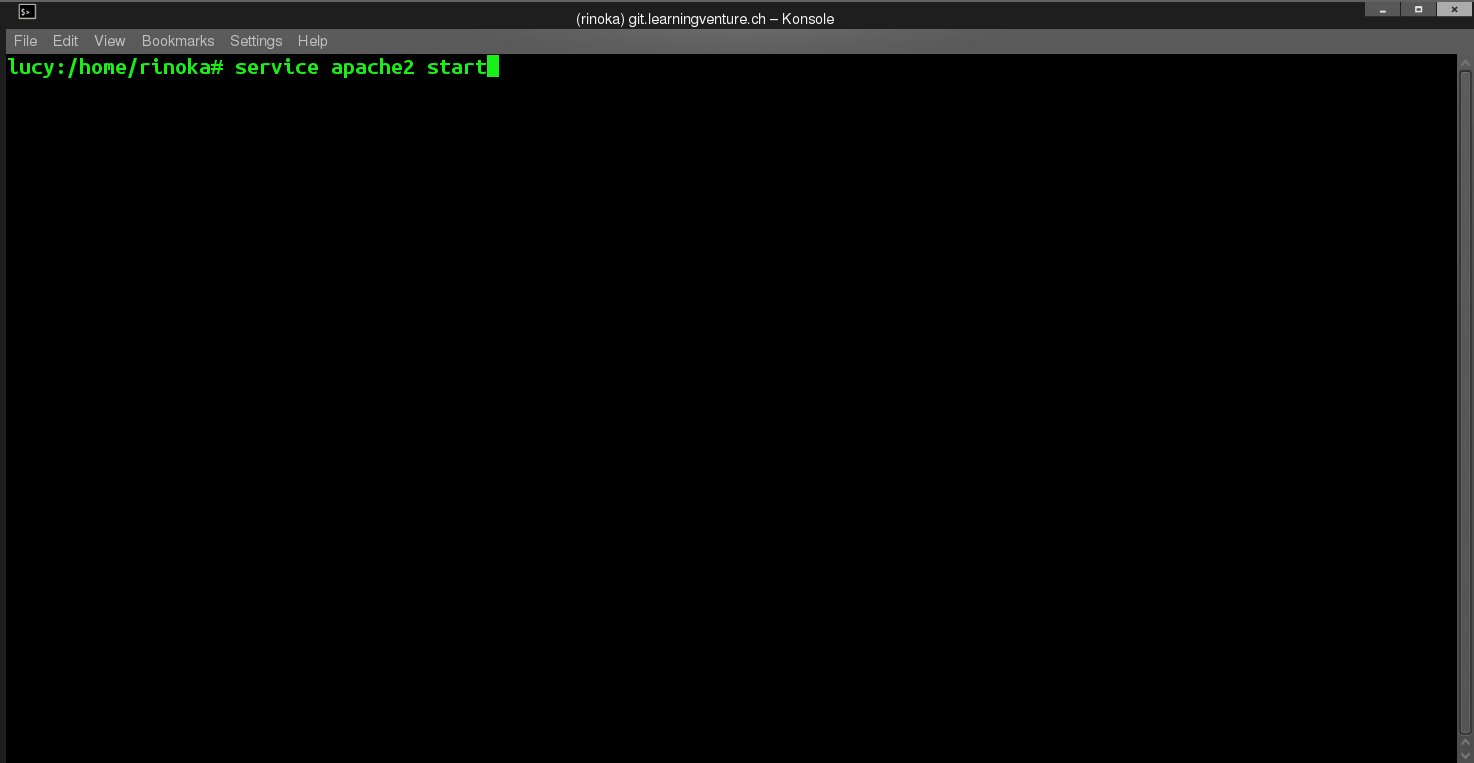
\includegraphics[width=13cm]{../Pics/start_apache}
	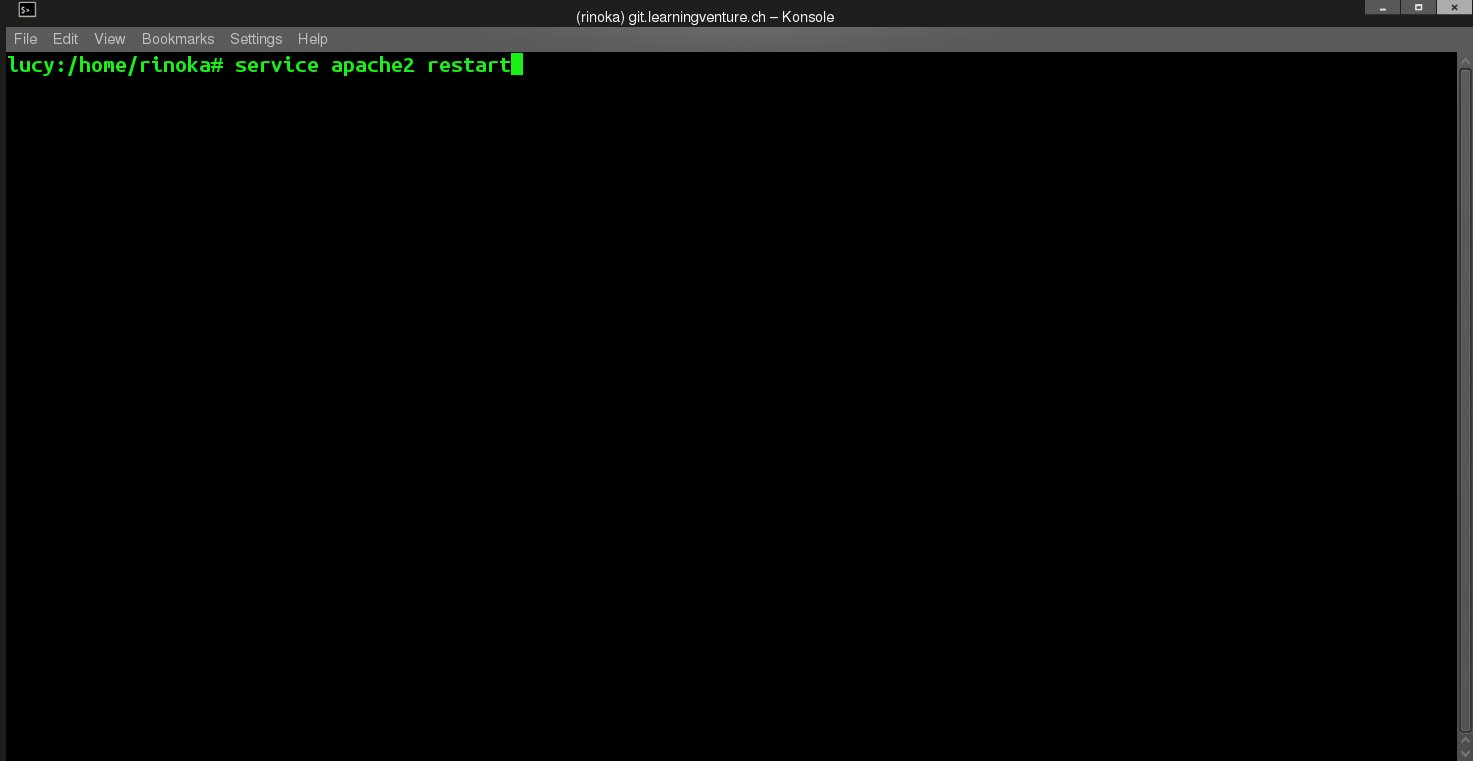
\includegraphics[width=13cm]{../Pics/apach2restart}
	\subsection{Linux}
	\subsection{Apache}
	Ausgnagslage gemäss Aufgabe:
	\newline
	Gemäss der im Auftrag erfordlichen Konfigurationsdateien muss die Wordpress-Installation auf dem Server unter folgendem Dateipfad installiert werden: /var/www/html/wordpress.
	\linebreak 
	\noindent\hspace*{5mm} Allerdings soll Wordpress auf IP-Adresse/blog aufgerufen werden. Dazu muss der VirtualHost in /etc/apache2/sites-available/ angepasst werden
	\subsection{MariaDB}
	Wir haben uns für \textit{\textbf{MariaDB}}  als Datenbank entschieden. Um diese zu Konfigurieren wird nach der Befehlsausführung zur Installation von MariaDB mit \textit{\textbf{lucy:/home/gilles\# apt-get install mariadb-client-10.0 mariadb-server-10.0 apache2 apache2-doc php5 php5-mysql libapache 2-mod-php5}} ein Fenster angezeigt, in dem man das Root-Passwort für die Datenbank festelegen soll.
	\newline
	\newline
	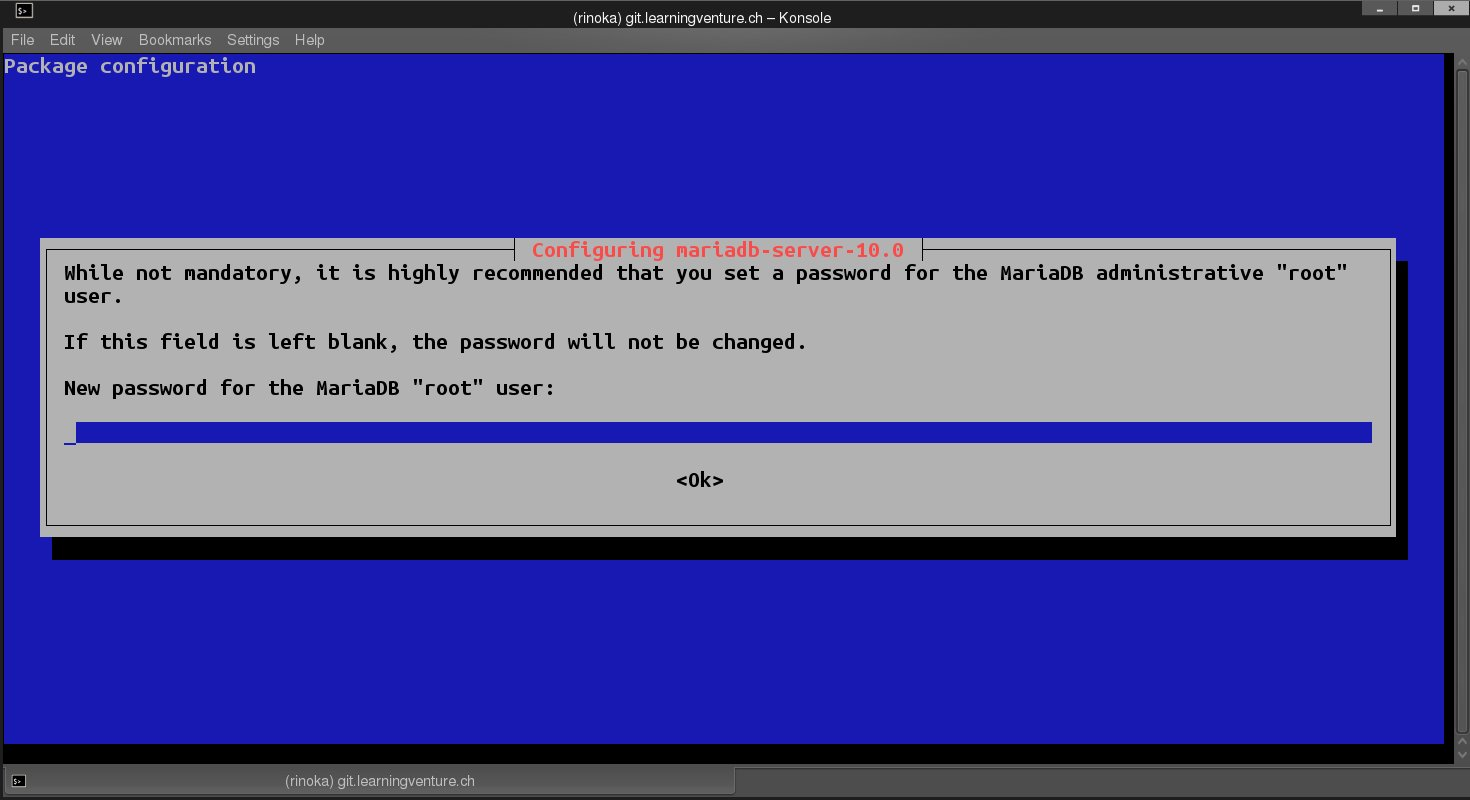
\includegraphics[width=13cm]{../Pics/3-lamp-stack-mariadb}
	\newline
	\newline
	Hier folgt natürlich nun die Datenbank erstellung, wie folgt:
	\subsection{PHP}
	\section{WordPress}
	\section{OwnCloud}
\end{document}